\section{Common approaches to the optimization problems}

To build the optimization problem it's necessary to model the system power and application, and controllable variables. Common approaches to the optimization problems are:

Minimize the energy function in function of our control variables, subject to constraints in the control variable.

\begin{equation}
\begin{aligned}
\textrm{min} \quad & P(s_1, s_2, ...)T(s_1,s_2,...)\\
\textrm{subject to} \quad & b_1<s_1<b_2\\
\quad & b_3<s_2<b_4\\
\quad & \vdots\\
\end{aligned}
\end{equation}

Another way is to minimize the total energy, with the constraint of to finish the work.

\begin{equation}
\begin{aligned}
\textrm{min} \quad & \sum{P_it_i}\\
\textrm{subject to} \quad & W_{tot} = \sum w_i\\
\quad & \vdots\\
\end{aligned}
\end{equation}

This kind of problem can be seen in multiple ways, considering an application as the total workload and choosing different speeds for each phase of the application, or could also treat each workload as a different application and create schedulers both CPU and cluster level. In fact the question of on each level of optimizer produces a better result is not well explored in the literature yet. The habitual approach it's to tackle each problem at once and combine the strategies resulting in a chain of schedulers.

The complexity of this problem also varies, depending on the choice of power function it can result in linear programming \cite{Kim2015RacingHeuristics}, quadratic programming \cite{Horyath2008Multi-modeClusters}, until NP-hard problems \cite{Fu2018RaceMinimization}.

\subsection{DVFS optimization} \label{sec:dvfs_optmin}
The effectiveness of the proposed approach for optimization was evaluated with a simple algorithm that finds the optimal frequency and number of active cores from the equation proposed. The results were then compared to the Linux default choices for power management.

With the equation developed \ref{eq:en_final}, it is possible to calculate energy consumption estimations for every possible configuration since there is a finite interval of possible values for the frequency and cores. Then, the configuration that minimizes energy consumption for a given input can be selected. It is also possible to apply constraints on the execution time, frequency, and the number of active cores.

Current HPC managers leave to the user the choice of how many cores to use. Because of that three situations were analyzed with relation to the number of cores:

\begin{enumerate}
	\item Worst choice: number of cores that maximize the total energy consumed
	\item Random choice: energy consumed for a random choice of number of cores
	\item Best choice: number of cores that minimize the total energy consumed (oracle)
\end{enumerate}

The default option for the Linux governor is the Ondemand, and by default, it does not have a DPM control for the number of active cores. Since Ondemand only does DVFS, to allow the comparison, each application was executed with all number of cores available in the system 1 to 32.

Figures \ref{fig:energy_worst_case}, \ref{fig:energy_mean_case} and \ref{fig:energy_best_case}, shows the energy savings with respect to Ondemand in the following way $\frac{Ondemand-Model_{min}}{Ondemand}$ with all three cases described above. The list below shows the savings and losses for each case:


\begin{figure}[ht]
	\centering
	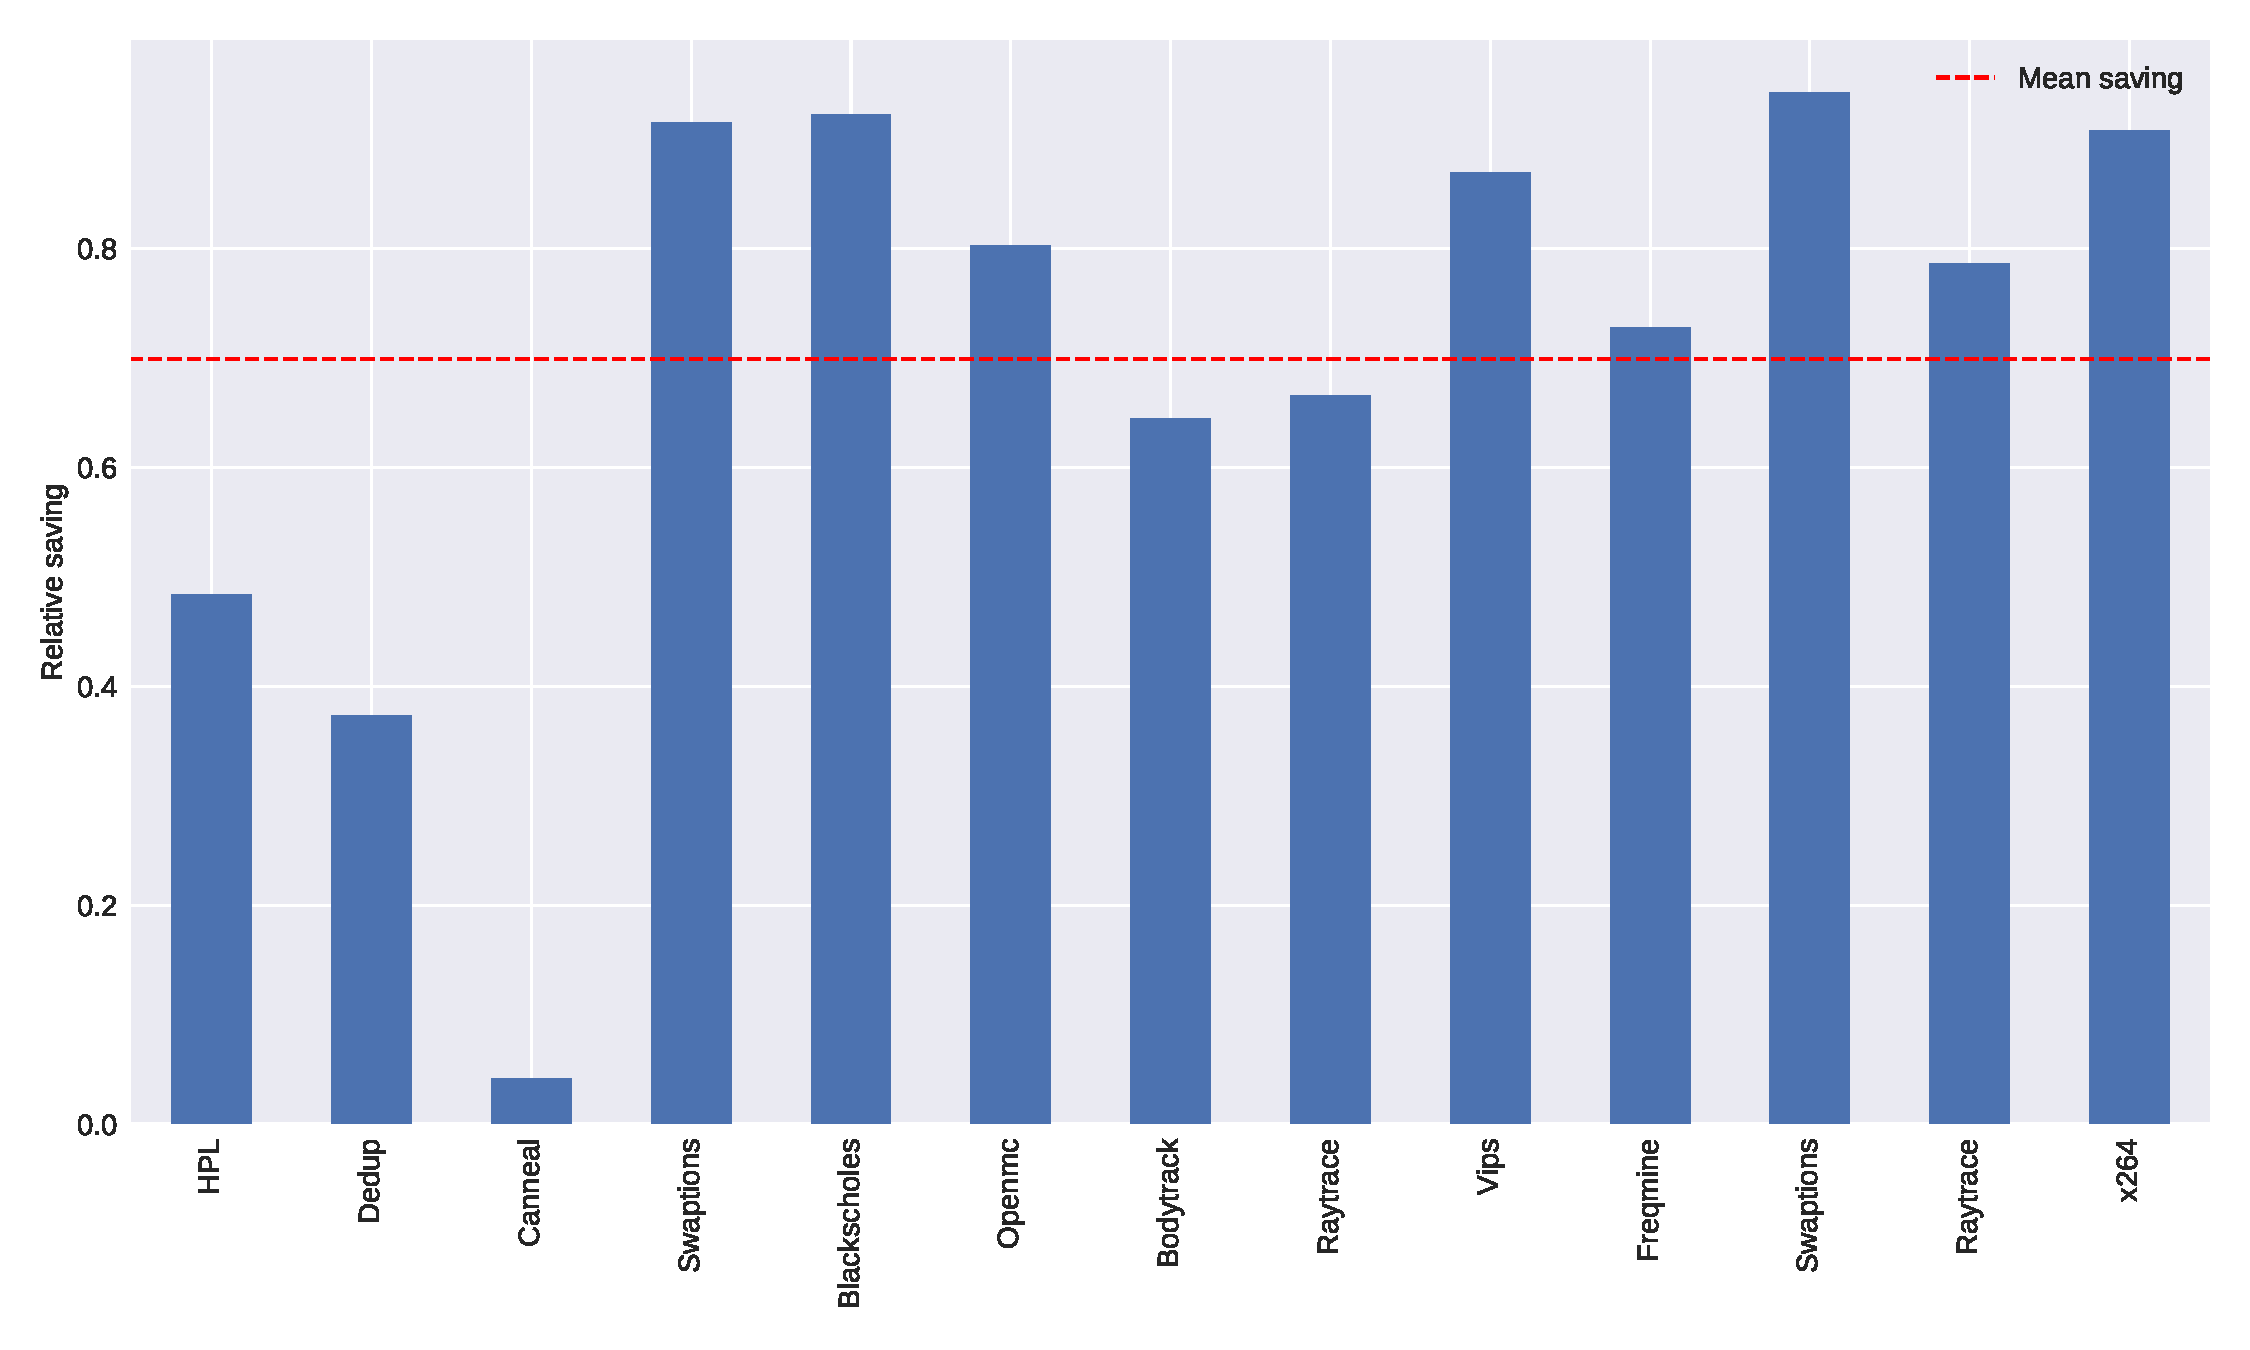
\includegraphics[width=\columnwidth,height=8.5cm]{models/figures/dvfs_cmp_max.png}
	\caption{Energy saving comparison with the proposed model and for the worst case}
	\label{fig:energy_worst_case}
\end{figure}

\begin{figure}[H]
	\centering
	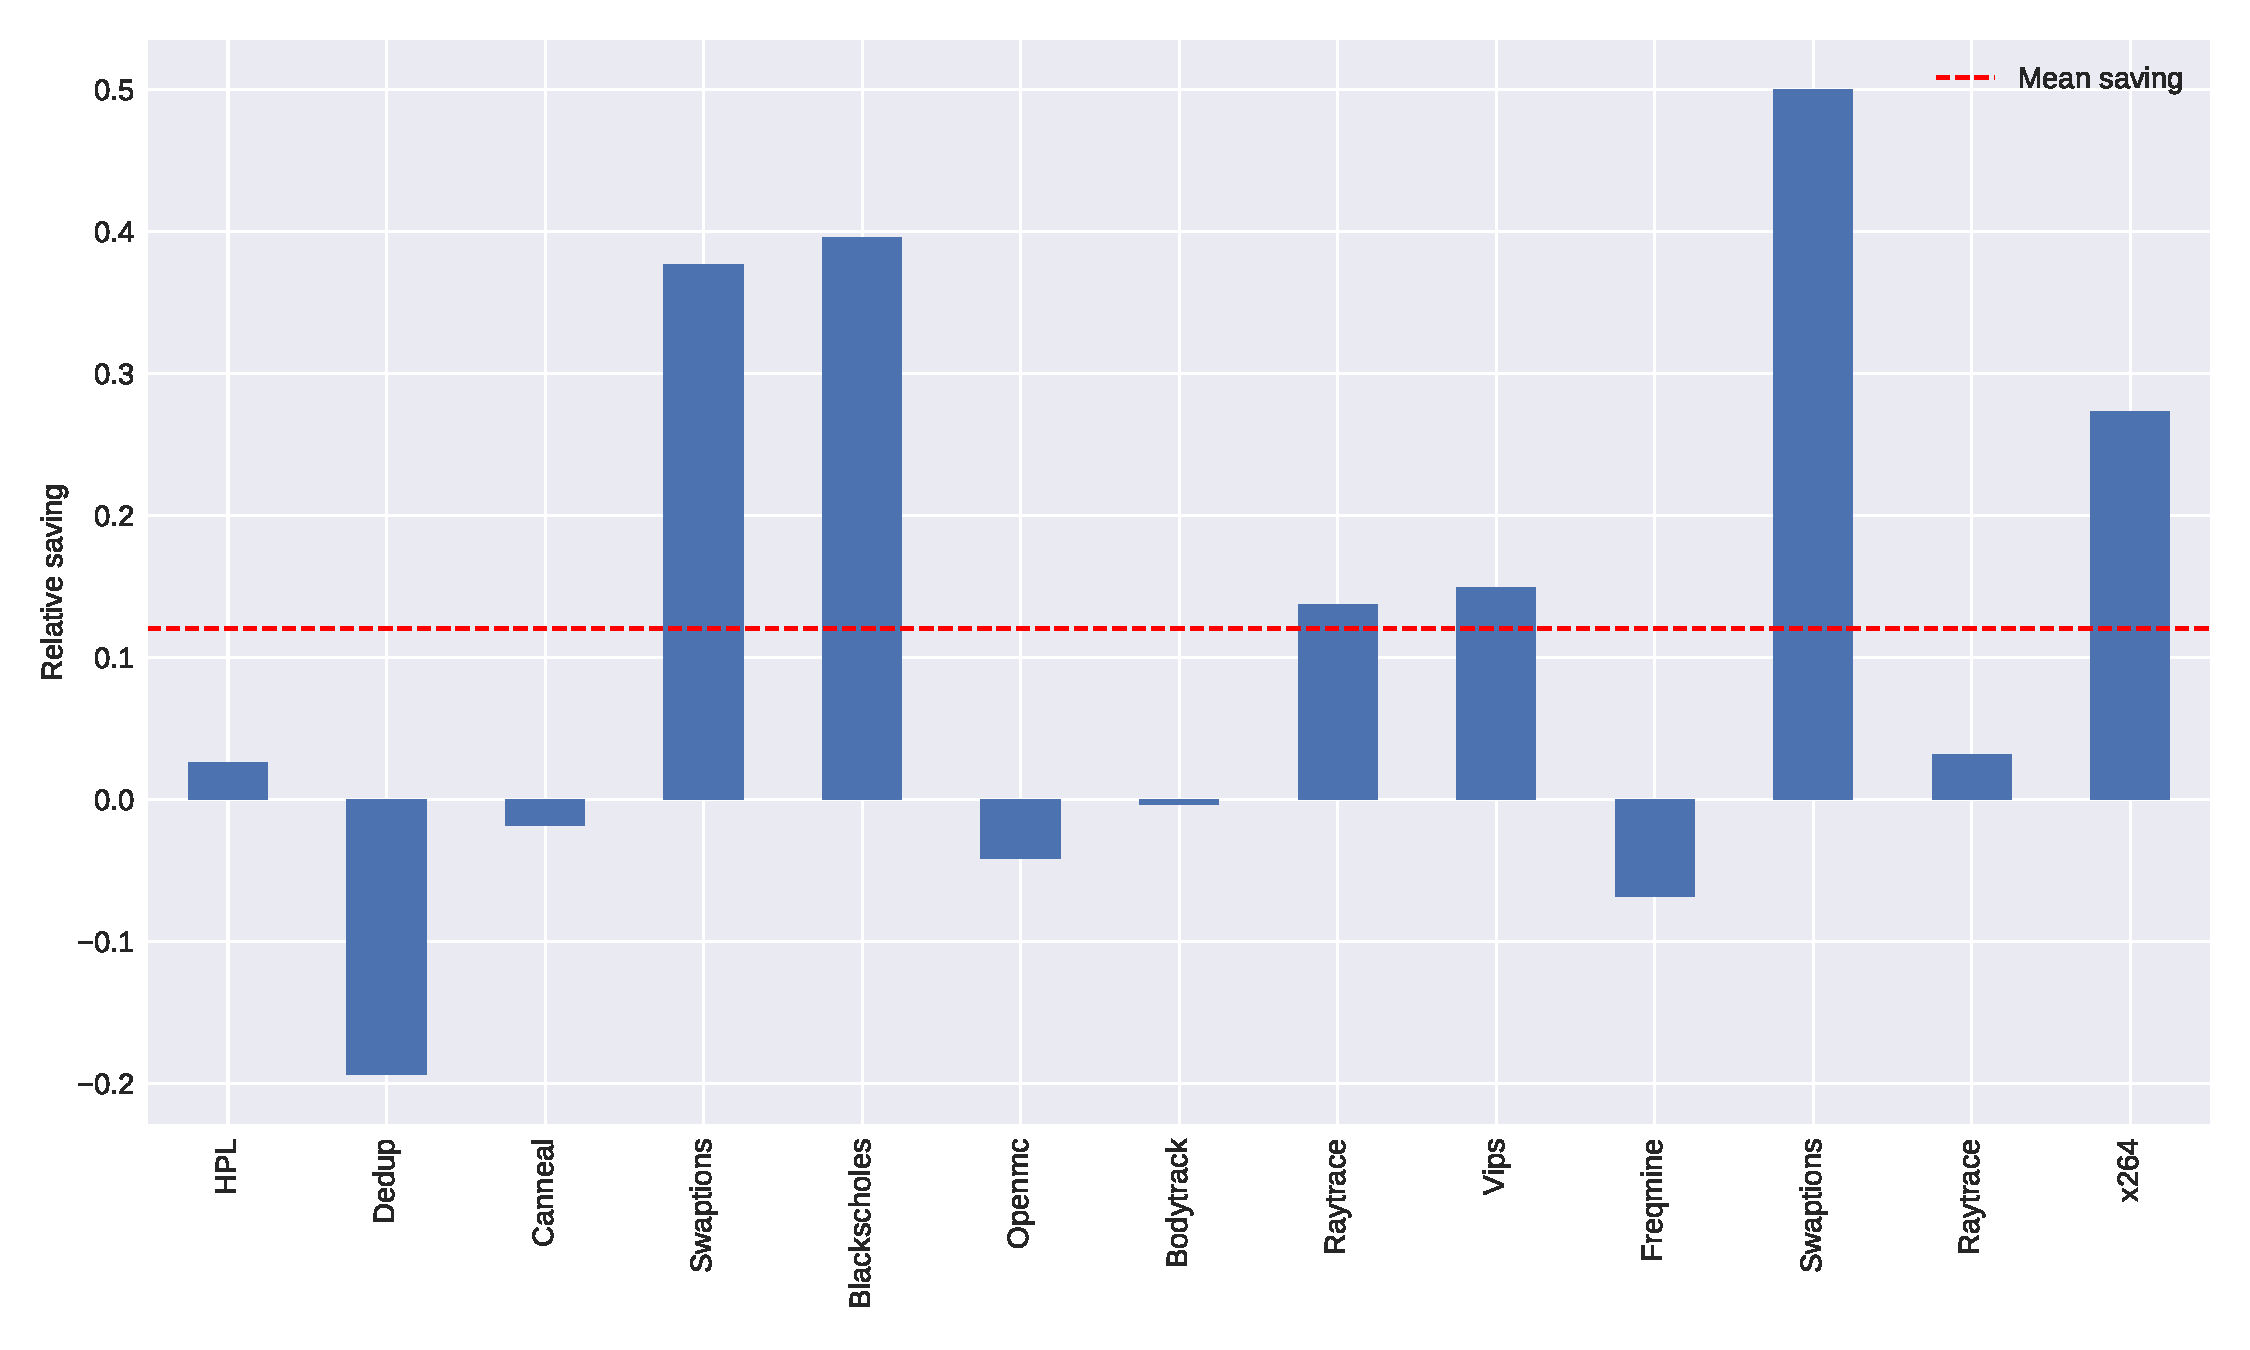
\includegraphics[width=\columnwidth]{models/figures/dvfs_cmp_mean.png}
	\caption{Energy saving comparison with the proposed model and for the random case}
	\label{fig:energy_mean_case}
\end{figure}

\begin{figure}[H]
	\centering
	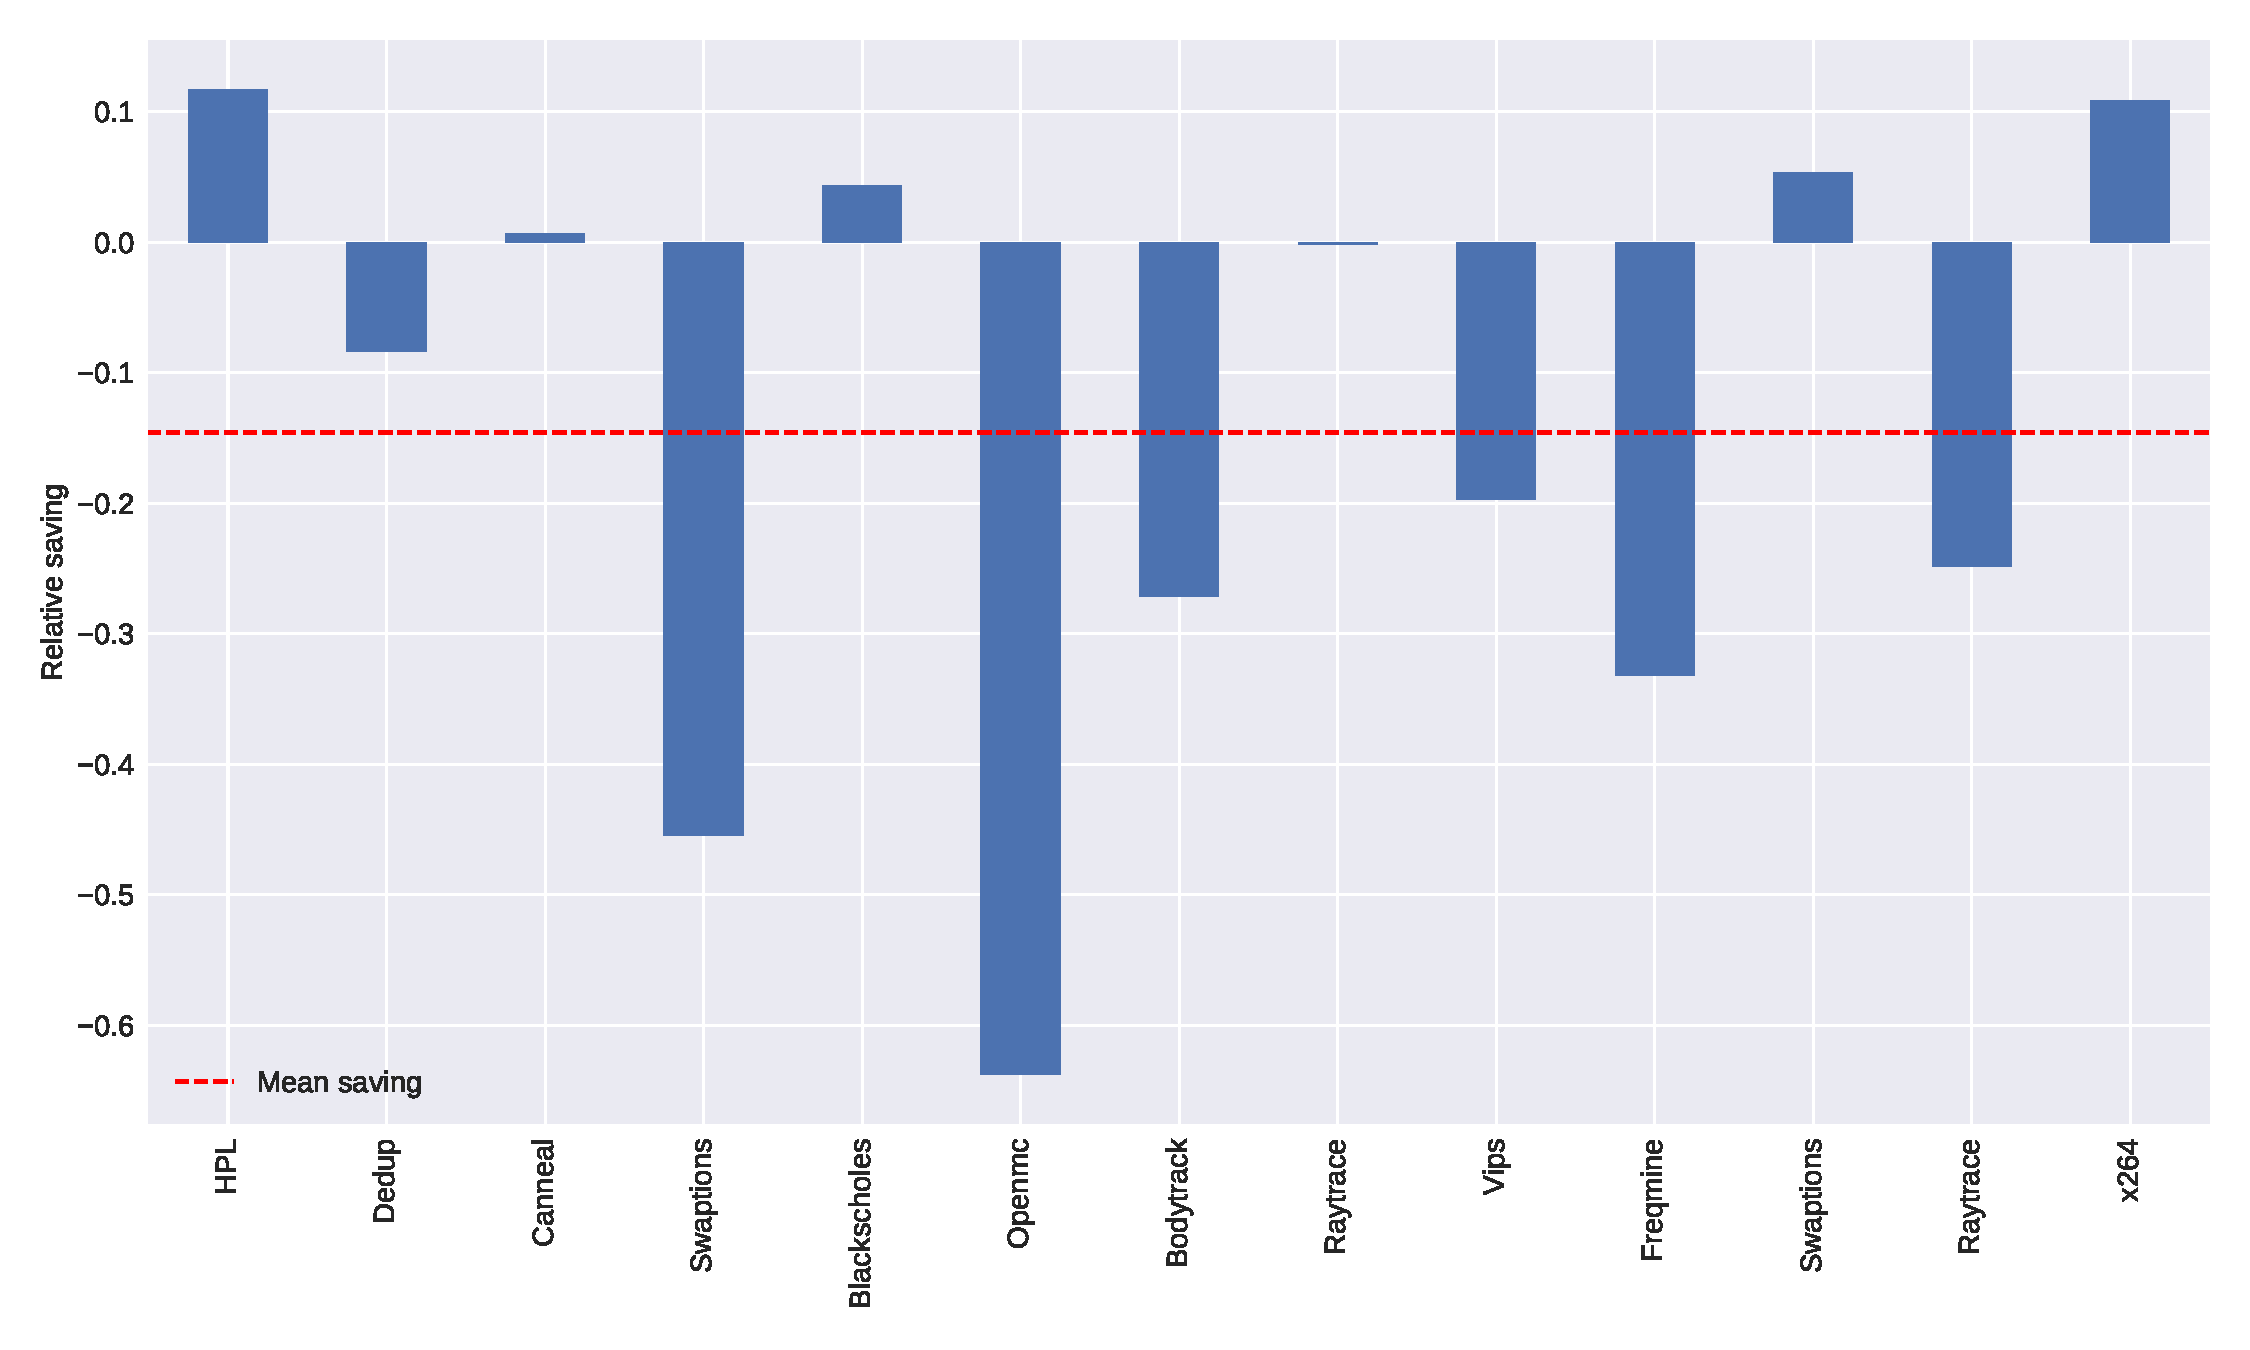
\includegraphics[width=\columnwidth]{models/figures/dvfs_cmp_32.png}
	\caption{Energy saving comparison with the proposed model and for the best case}
	\label{fig:energy_best_case}
\end{figure}

The list below shows the savings and losses for each case:

\begin{enumerate}
	\item Worst choice: save 69.88\% on average
	\item Random choice: save 12.04\% on average
	\item Best choice: lost 14.06\% on average
\end{enumerate}

%This can be explained by the linear speedup characteristic from this application. Thus, it is to be expected that on constant efficiency, the better solution will be with more cores.

%The other results on the other applications show that the proposed approach, even in cases on the bests configurations for DVFS, demonstrate that can obtain energy saving of up 18\%, comparing to the Ondemand governor.

%\begin{figure}[H]
%    \centering
%    \includegraphics[width=\columnwidth]{dvfs/completo_black_ondemand_nolimit_2_10.png}
%    \caption{Caption}
%    \label{fig:my_label}
%\end{figure}
%
%In general, for the case-study applications and case-study architecture, the optimal-energy configurations tend to be the ones using the highest frequency, which characterizes a race-to-idle rather than a pace-to-idle optimal behavior~\cite{Kim2015RacingHeuristics}. This can be explained by the large static power observed in the considered architecture, evidenced by the large $c_3$ parameter in (\ref{eq_power_final}) that was fitted in (\ref{eq:fittedpower}). With a large static power, using a pace-to-idle strategy, i.e. the use of frequencies lower than the maximum, is expected to be effective only if the sum of the leakage and the dynamic power parcels is larger than the static power parcel. 
%Based on the fitted power model, this would never happen, i.e. the sum of leakage and dynamic power is always less than the static power,
%\begin{equation*}
%p(0.29f^3+0.97f)+9.18s < 198.59, 
%\end{equation*}
%even if we use the maximum number of cores, $p=32$ and $s=2$, and the maximum frequency, $f=2.2$.
%Nevertheless, race-to-idle was not always the best strategy because energy scales with the execution time, which in turn scales inversely with the number of active cores and the operating frequency, and because power scales linearly with the number of cores, but exponentially with the frequency.
%
%The optimal number of active cores depends on the parallel scalability of the application. The more scalable the application, the more cores it requires to minimize energy. A scalable application can increasingly exchange the speedup of more cores with lower frequencies in order to spend less energy. This is because of the linear relationship between power and number of cores and the exponential relationship between power and frequency.
%
%In all cases, the method proposed here outperformed the worst case of the Ondemand governor. On average, the difference in energy consumption was about 790\%, being 1298\% the maximum difference and 59\% the minimum. In general, the energy consumption of the DFVS scheme was larger for smaller numbers of cores. Nonetheless, it was not always the case that the best number of cores for this scheme was the maximum, i.e. 32 cores. Possibly, for architectures with larger number of cores, choosing the exact number the minimizes energy consumption would be less evident.

Since the number of cores in HPC is requested by the user, the number of CPU requests during one year in UFRN's cluster was analyzed. The result is plotted in the figure \ref{fig:cpu_requests}.
\begin{figure}[H]
	\centering
	\includegraphics[width=\columnwidth]{models/figures/cpu_request.png}
	\caption{Number of CPUs requested by the users during 2016-2017}
	\label{fig:cpu_requests}
\end{figure}

The worst choice was always with a single core and is the most common choice of many regular users. The best choice was quite often 32 cores, which is the third most popular choice of the users but it is $72\times$ less than 1 core. This can point a direction of how much energy can be saved by using this technique for DPM or more advanced optimization algorithms that can be derived from our model.

In practice, this approach can be brought into production by allowing the resource manager to perform these changes for the user using pre-scripts and post-scripts for job submissions with energy consumption requirements. This approach is simple to be implemented and can work in almost any Linux system.


\section{Conclusion} \label{sec:conclusion}
This work proposes an energy model based on the frequency and number of cores for a full shared memory system. This model can serve as a base for DVFS and DPM optimization problems that include both frequency and active cores, as well for analysis of the contribution of each parameter (ex: parallelism level) to the energy consumption.

Results from 3 HPC benchmarks running in one cluster demonstrate the potential of the proposed novel model. While consuming less energy than traditional machine learning approaches, it can serve as bases from DVFS and DPM algorithm as shown in the \ref{sec:dvfs_optmin} in an average case saving about 12\% up to 69\%. The previous knowledge of the application's performance can expose sufficiently relevant information, such as parallel speedups, that is harder to guess in run-time techniques based on DVFS.

A weakness of the proposed model is the need for information about the input size of the application that can be complex to derive. A possible solution would be to precisely define what is input size, given an definition in function of common variable for all applications like throughput for example. Future work will demonstrate all the possible analysis that is possible to archive with the equation as long as more advanced DVFS models that can be derived using the equation. For instance identification of different phases of the target program and thus, it will enable more fine-grained changes of the frequency and, perhaps, the number of active cores, to further improve the results presented here.

Another important aspect that is typically not taken into account is the number of processing cores to be used by a parallel program. This choice is left to the user, which often is not trivial as shown in this paper.


%%%% moved to the conclusions.
% A weak of this approach is that the model of performance and power needed to be trained with previously known input sizes. This weakness can be treated with a future solution that can incorporate a prediction of input size during execution of the application. 

